\documentclass[12pt,dvipdfmx,svgnames,a4paper,uplatex]{ujreport}
% \documentclass[12pt,dvipdfmx,svgnames,a4paper,uplatex, draft]{ujreport}  % 画像を省略してコンパイルを高速化する
% +++++++++++++++++++++++++++++++++++++++++++
% パッケージの導入
% +++++++++++++++++++++++++++++++++++++++++++
%
% ===========================================
% 原稿設定
% ===========================================
\usepackage[normalem]{ulem}  % 卒論の二行組タイトルに下線をつける
% 表紙用スタイルファイル
% \usepackage{hyoshi_bachelor}  % 卒論用
\usepackage{hyoshi_master}    % 修論用
% 原稿のサイズ
\usepackage[top=25truemm,bottom=25truemm,left=25truemm,right=25truemm]{geometry}
% \usepackage{relsize}
%
% ===========================================
% 図・表関係
% ===========================================
\usepackage{graphicx}
\graphicspath{{./pics/}}  % \includegraphicsで参照するディレクトリ
%これを \graphicspath{{./pics/}, {/path/to/figure/directory/}} のように書けば複数のディレクトリの画像を参照できる.
%
% ===========================================
% 参考文献
% ===========================================
\usepackage[
  backend=biber,  % 文献ソートを担当(登場順なので不要?)
  style=phys,  % AIPとAPSのスタイル
  biblabel=brackets,  % 文献番号を [1] のように表記
  pageranges=false]{biblatex}  % 文献のページ範囲を省略
\addbibresource{../bib_textbooks.bib}  % 教科書など
\addbibresource{../bib_articles.bib}  % 論文など(※Mendeleyで自動生成)
% \addbibresource{/path/to/hogehoge.bib}  % 他にも追加可能
%
% ===========================================
% chapterごとの改ページを抑制
% ===========================================
\makeatletter
\renewcommand{\chapter}{%
  \if@openright\cleardoublepage\fi
  \thispagestyle{jpl@in}%
  \global\@topnum\z@
  \@afterindenttrue
  \secdef\@chapter\@schapter}
\makeatother
%
% ===========================================
% 独自スタイルの定義
% ===========================================
\usepackage{../mystyle}
\usepackage[english]{babel}  % arabic数字でページ番号を指定
\renewcommand{\thefootnote}{\fnsymbol{footnote}}
\usepackage{lipsum}  % ダミー文章
\usepackage{bxjalipsum}  % 日本語のダミー文章
%
% ===========================================
% 表紙の記述
% ===========================================
\title{
  論文タイトル一行目 \\
  論文タイトル二行目
}
\date{20〇〇年2月}
\author{阪大~太郎}

% +++++++++++++++++++++++++++++++++++++++++++
% 本文
% +++++++++++++++++++++++++++++++++++++++++++
\begin{document}
\maketitle

% ===========================================
% 概要(英語) *****修士論文のみ(卒論は緒言)*****
% ===========================================
\pagenumbering{roman}
\documentclass[11pt,dvipdfmx,svgnames,a4paper,uplatex]{ujarticle}
% +++++++++++++++++++++++++++++++++++++++++++
% パッケージの導入
% +++++++++++++++++++++++++++++++++++++++++++
%
% ===========================================
% 原稿設定
% ===========================================
% 原稿のサイズ
\usepackage[top=25truemm,bottom=25truemm,left=25truemm,right=25truemm]{geometry}
\setlength\intextsep{0pt}
\setlength\textfloatsep{0pt}
\usepackage{relsize}
\usepackage{setspace}
\onehalfspacing
\usepackage[compact]{titlesec}
\titleformat{\section}{\normalfont\bfseries}{\thesection}{1em}{}  % \sectionのフォントサイズを本文と統一
\titlespacing*{\section}{0pt}{*0}{0pt}  % section前後のスペーシングをなくす
\pagestyle{empty}
% 一行あたり文字数と一ページあたり行数の指定
\makeatletter
\def\mojiparline#1{
    \newcounter{mpl}
    \setcounter{mpl}{#1}
    \@tempdima=\linewidth
    \advance\@tempdima by-\value{mpl}zw
    \addtocounter{mpl}{-1}
    \divide\@tempdima by \value{mpl}
    \advance\kanjiskip by\@tempdima
    \advance\parindent by\@tempdima
}
\makeatother
\def\linesparpage#1{
    \baselineskip=\textheight
    \divide\baselineskip by #1
}
%
% ===========================================
% 図・表関係
% ===========================================
% \usepackage[draft]{graphicx}
\usepackage{graphicx}
\usepackage{wrapfig}  % 文章に囲まれた図の挿入
\graphicspath{{../thesis/pics/}}  % \includegraphicsで参照するディレクトリ
%これを \graphicspath{{../thesis/pics/}, {/path/to/figure/directory/}} のように書けば複数のディレクトリの画像を参照できる.
\usepackage{setspace,caption}
\captionsetup[figure]{font={stretch=0.8}}  % 図のキャプションのスペーシングを縮める
%
% ===========================================
% 参考文献
% ===========================================
\usepackage[backend=biber,style=phys,biblabel=brackets,pageranges=false,maxbibnames=3,doi=false]{biblatex}
\setlength\bibitemsep{0.0\baselineskip}
\addbibresource{../bib_textbooks.bib}  % 教科書など
\addbibresource{../bib_articles.bib}  % 論文など
\AtEveryBibitem{\clearlist{language}}  % 文献の言語情報を出力しない
%
% ===========================================
% 独自スタイルの導入
% ===========================================
\usepackage{../mystyle}
\renewcommand{\figurename}{Fig.}
\usepackage{bxjalipsum}
\DeclareSourcemap{
  % 論文のタイトルを非表示(mystyle.styで論文のタイトル表示からダブルクォーテーションを削除,という指示をしているのでここに書く)
  \maps[datatype=bibtex]{
    \map{
      \pertype{article}
      \step[fieldset=title, null]
    }
  }
}
%
% ===========================================
% 表紙の記述
% ===========================================
\title{\underline{title}}
\author{name}
\date{\today}

% +++++++++++++++++++++++++++++++++++++++++++
% 本文
% +++++++++++++++++++++++++++++++++++++++++++

\begin{document}
\mojiparline{42}  % 一行あたり文字数
\linesparpage{38}  % 一ページあたり行数

\centerline{\textbf{
  修士論文のタイトル修士論文のタイトル修士論文のタイトル修士論文のタイトル
}}
\rightline{阪大~太郎}

% ===========================================
\section{緒言}
% ===========================================

\begin{wrapfigure}{r}{12zw}
  \vspace*{-\intextsep}
  \centering
  \includegraphics[width=10zw]{example-image-9x16}
  \caption{
    Figure caption figure caption figure caption.
  }
  \label{fig:intruduction}
  \vspace*{-\intextsep}
\end{wrapfigure}

\textcolor{LightGray}{
\jalipsum[1-2]{wagahai}
}


% ===========================================
\section{実験手法}  % 自身の研究に合わせて変更
% ===========================================

\begin{wrapfigure}{r}{26zw}
  \vspace*{-\intextsep}
  \centering
  \includegraphics[width=24zw]{example-image-16x9}
  \caption{
    Figure caption figure caption figure caption figure caption figure caption figure caption figure caption.
  }
  \label{fig:intruduction}
  \vspace*{-\intextsep}
\end{wrapfigure}

\textcolor{LightGray}{
\jalipsum[3]{wagahai}
\jalipsum[4]{wagahai}
}


% ===========================================
\section{実験結果}  % 自身の研究に合わせて変更
% ===========================================

\begin{figure}[htb]
  \centering
  \subfloat[\(f (\vb*{x},t)\)]{
    \includegraphics[width=0.24\textwidth]{example-image-1x1}
    \label{subfig:f}
  }
  \subfloat[\(g (\vb*{x},t)\)]{
    \includegraphics[width=0.24\textwidth]{example-image-1x1}
    \label{subfig:g}
  }
  \subfloat[\(h (\vb*{x},t)\)]{
    \includegraphics[width=0.24\textwidth]{example-image-1x1}
    \label{subfig:h}
  }
  \subfloat[\(i (\vb*{x},t)\)]{
    \includegraphics[width=0.24\textwidth]{example-image-1x1}
    \label{subfig:i}
  }
  \caption{
    Figure caption figure caption figure caption figure caption figure caption figure caption figure caption figure caption figure caption figure caption.
  }
  \label{fig:fig_result}
\end{figure}

\textcolor{LightGray}{
\jalipsum[5]{wagahai}
}


% ===========================================
\section{結言}
% ===========================================

私は,〇〇〇という問題に注目し~\cite{Goto2017a,GotoJPS2018},〜〜〜を明らかにした~\cite{Araki_master_thesis}.

% ===========================================
\printbibliography[title=参考文献]
% ===========================================

\end{document}

\clearpage

% ===========================================
% 目次
% ===========================================
\renewcommand{\contentsname}{目次}
\tableofcontents
\clearpage

% ===========================================
% 記号表
% ===========================================
\chapter*{記号表}

\section*{パラメータ,無次元量}
\begin{tabular}{lll}
\(\pi\)  & : & 円周率 \\
\(\nu\)  & : & 動粘性係数 \\
\(\rho\) & : & 密度 \\
\(\mathrm{Re}\) & : & Reynolds数
\end{tabular}

\section*{物理量}
\begin{tabular}{lll}
\(L\) & : & 乱流の特徴長さ \\
\(U\) & : & 乱流の特徴速度 \\
\(T\) & : & 乱流の特徴時間スケール \\ \hline
\(\vb*{u}=(u,v,w)\)  & : & 流速 \\
\(p\) & : & 圧力 \\
\(\epsilon\) & : & エネルギ散逸率 \\
\(\varPi\) & : & エネルギ流束 \\ \hline
\(\vb*{x}=(x,y,z)\) & : & 大域座標 \\
\(\vb*{\xi}=(\xi_1,\xi_2)\) & : & 局所座標 \\
\(t\) & : & 時刻
\end{tabular}

\section*{関数,演算子}
\begin{tabular}{lll}
\(Cor\qty[A,B]\qty(\alpha)\) & : & \(A\)と\(B\)の\(\alpha\)に関する相関関数 \\
\(\delta_{ij}\) & : & Kroneckerのデルタ \\
\(\expval{(\cdot)}\) & : & 空間平均 \\
\(\overline{(\cdot)}\) & : & 時間平均 \\
\(\mathcal{A}\) & : & 局所座標と大域座標を結ぶ写像
\end{tabular}

\section*{上付き・下付き文字}
\begin{tabular}{lll}
  \((\cdot) ~^e\) & : & 局所座標系の量 \\
  \((\cdot)_l \equiv \underline{(\cdot)^e}\) & : & 局所座標を並べた量 \\
  \((\cdot)_g \equiv \mathcal{A} (\cdot)_l\) & : & 大域座標の量 \\
\end{tabular}

\clearpage

% ===========================================
% 以降は日本語環境
% ===========================================
\renewcommand{\figurename}{図}
\renewcommand{\tablename}{表}
\renewcommand{\prechaptername}{第}
\renewcommand{\postchaptername}{章}

% ===========================================
% 緒言 *****卒業論文のみ?(修論は英語概要)*****
% ===========================================
\pagenumbering{arabic}  % 以降算用数字でページ番号を記述
% \chapter{緒言}
\label{chap:Introdunction}

緒言をここに執筆.
修論では英語で要旨を書くので要らないかも?
研究背景などは次章でまとめればよい.

\textcolor{LightGray}{
\jalipsum[1-4]{wagahai}
}


% ===========================================
% 研究背景
% ===========================================
\chapter{乱流の統計的普遍則と動力学}
\label{chap:StatisticalUniversalityAndDynamicsOfTurbulence}
% prefix: SUADOT

本章では,今日の乱流理論の基礎となっているKolmogorovの理論を,局所平衡仮説を軸にまとめる.
まず~\ref{sec:TurbulenceAndEnergyCascadePicture}節で乱流とその現象論的描像であるエネルギカスケード描像を導入する.


\section{乱流とエネルギカスケード描像}
\label{sec:TurbulenceAndEnergyCascadePicture}

乱流とは流体が時空間的にきわめて乱れたふるまいをする現象であり,身の回りのいたるところでみられる.
乱流を普遍的に記述することは理学的にも工学的にも重要な問題であり,長年に渡り膨大な研究がおこなわれてきた~\cite{tennekes1972first,Landau1987Fluid,KidaYanase,frisch1995tlk}.

非圧縮流体の運動は,Navier-Stokes方程式と非圧縮条件
\begin{empheq}[left=\empheqlbrace]{align}
  \pdv{\vb*{u}}{t} + \qty(\vb*{u} \cdot \grad) \vb*{u} &= - \grad p + \frac{1}{\Re} \laplacian \vb*{u}
  \label{eq:LEHASU_NavierStokesEq} \\
  \div \vb*{u} &= 0
  \label{eq:LEHASU_InCompressibility}
\end{empheq}
で記述される.
これらの方程式は流れのマクロな特徴速さスケール\(U\)と特徴長さスケール\(L\)で無次元化されており,無次元量であるReynolds数
\begin{equation}
  \Re \equiv \frac{UL}{\nu}
  \label{eq:LEHASU_DefOfReynoldsNumber}
\end{equation}
に支配されている.
ただし,\(\nu\)は流体の動粘性係数である.
\(\Re\)は流体に作用する慣性と粘性の比,非線形項と線形項の比,あるいは流れに注入されるエネルギ流束の大きさを表すパラメータなどと表現される~\cite[p.~8,p.~409]{Tatsumi}.
一般に,\(\Re\)が\(\order{10^3}\)を超えると流れは乱流となる.

乱流を説明する現象論として,Richardsonの提唱したエネルギカスケード描像がある~\cite{Goto2017a,GotoJPS2018}.
その模式図を~\ref{fig:EnergyCascade_Schematic.pdf}に示す~\cite{gotolab}.
\begin{figure}[!t]
  \centering
  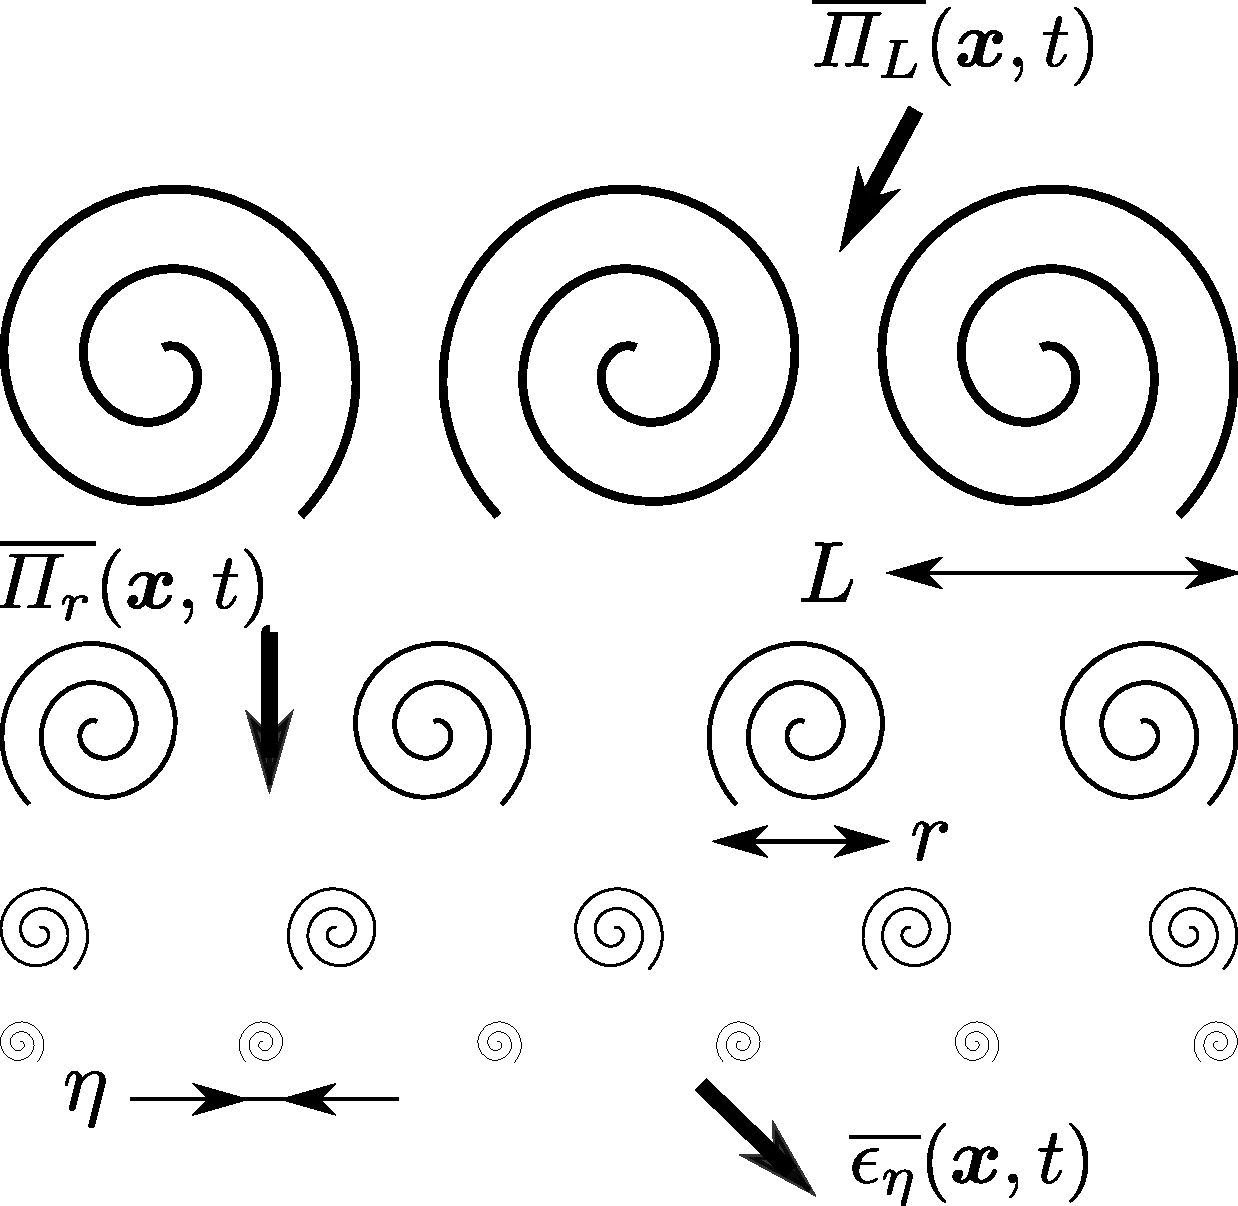
\includegraphics[bb=0.000000 0.000000 594.189270 578.870117, width=0.6\textwidth]{EnergyCascade_Schematic.pdf}
  \caption{
    エネルギカスケード描像の模式図.
    図の上部が大スケール渦,下部が小スケール渦を表し,エネルギが大スケールから小スケールに(上から下に)「カスケード」する様子を模式的に示している.}
  \label{fig:EnergyCascade_Schematic.pdf}
\end{figure}
この描像は,乱流をさまざまなスケールの渦を用いて説明する.
まず,境界条件や外力によって,マクロな長さスケール\(L\)程度の渦にエネルギが注入される.
エネルギを持った大スケール渦は,自身より小さな渦を生成しこれにエネルギを伝達する.
このエネルギ伝達が繰り返しおこなわれることで,エネルギが漸次より小さなスケールに「カスケード」する.
粘性が支配するスケール\(\eta\)程度の渦に伝達されたエネルギは,熱として散逸する.
エネルギカスケードは次節以降で述べるKolmogorovの乱流理論の骨子となる重要な描像である.


% ===========================================
% 室内実験
% ===========================================
\chapter{粒子画像流速測定による室内実験}
\label{chap:Experiment}

本章では,閉じた系の乱流を粒子画像流速測定(PIV)実験で測定した結果を報告する.
\ref{sec:ExperimentalSetup}節で実験装置の諸元についてまとめる.


\section{実験装置}
\label{sec:ExperimentalSetup}

実験装置の模式図を図~\ref{fig:experiment_schematic}に,実験に使用する機材の一覧を表~\ref{table:ListofEquipment}に示す.
\begin{figure}[!t]
  \centering
  \includegraphics[width=0.6\textwidth]{example-image-16x9}
  \caption{
    三次元CADによる実験装置の模式図.
  }
  \label{fig:experiment_schematic}
\end{figure}

\begin{table}[!t]
  \centering
  \caption{実験機材の一覧}
  \begin{tabular}{c|cc}
    機材名称 & メーカー & 型番 \\ \hline \hline
    円筒容器 & アクリル製 & 加工品 \\
    回転円盤 & 樹脂製 & 加工品 \\
    サーボモータ & オリエンタルモーター社製 & NX940AS--PS5 \\
    モータ制御用ソフトウェア & オリエンタルモーター社製 & MEXE02 \\
    ハイスピードカメラ & BASLER社製 & acA 1920--150 \si{\micro \meter} \\
    脱気装置 & ERC社製 & ERC--3302W \\
    ロッドレンズ & シグマ光機社製 & RODB--05L10 \\
    ミラー & シグマ光機社製 & TFA--10S05--10 \\
    プリズム & シグマ光機社製 & PRB2--10--550 \\
    平面球凸レンズ & シグマ光機社製 & SLB--30--800P
  \end{tabular}
  \label{table:ListofEquipment}
\end{table}


\subsection{系の無次元化}
\label{subsec:ES_UndimentionalizedSystem}

円盤の半径\(D/2\, \si{m}\)と回転円盤の外周速度\(U\, \si{m/s}\)より,Reynolds数
\begin{equation}
  \Re \equiv \frac{UD/2}{\nu}
  \label{eq:ES_DefOfReynoldsNumber}
\end{equation}
を定義する.
ただし,外周速度\(U\)は円盤の回転周期\(T\, \si{s}\)と半径\(D/2\)をもちいて
\begin{equation}
  U \equiv \frac{2\pi D/2}{T}
  \label{eq:ES_DefOfVelocityAtRim}
\end{equation}
で表せる.
このとき,Reynolds数の定義は
\begin{empheq}{align}
  \Re &\equiv \frac{UD/2}{\nu} \nonumber \\
    &= \frac{\pi D^2}{2\nu T}
  \label{eq:ES_DefOfReynoldsNumber_T}
\end{empheq}
となる.
作動流体である水の動粘度は\(\nu = 1.0 \times 10^-6\, \si{m^2/s}\)とする.
実験で変化させるのは\(T\)のみであり,例えば\(T=2.0\, \si{s}\)のとき,Reynolds数は
\begin{empheq}{align}
  \Re &= \frac{\pi D^2}{2\nu T} \\
    &= \frac{\pi \times (0.200)^2 }{2 \times 1.0\times 10^{-6} \times 2.0} \fallingdotseq 3.1 \times 10^4
\end{empheq}
となる.


% ===========================================
% 数値計算
% ===========================================
\chapter{スペクトル要素Fourier法による直接数値計算}
\label{chap:NumericalCalculation}

本章では,スペクトル要素Fourier法により平滑円盤で駆動されるvon K\'arm\'an流を直接数値計算(DNS)した結果を報告する.
\ref{sec:BasisOfSpectralElementMethod}節では,スペクトル要素法の基礎をまとめる.
\ref{sec:SpectralElementFourierMethod}節では,円柱座標系で周方向に一次元Fourierスペクトル法,軸および半径方向に二次元スペクトル要素法を用いたスペクトル要素Fourier法のアルゴリズムをまとめる.


\section{スペクトル要素法の基礎}
\label{sec:BasisOfSpectralElementMethod}

乱流の数値計算にはさまざまな手法が用いられる.
スペクトル法とは適切な性質をもつ基底関数により物理量を波数空間に展開することを通じて問題を解く手法であり,高精度な半面領域形状が単純なものに制約される~\cite{Ishioka_spectral}.
これに対し,複雑な形状の問題には空間を離散化し隣接する座標点の情報を用いる差分法~\cite{Kajishima_turbulence_simulation}や方程式を弱形式で定義し空間を離散化した「要素」の接点の情報を用いる有限要素法などが広く用いられている~\cite{1994fem_mathematics}.
スペクトル要素法とは,1980年代に提唱された「スペクトル法の精度と有限要素法の一般性を融合した\footnote{``combines the generality of the finite element method with the accuracy of spectral techniques''~\cite{Patera1984}}」計算手法である~\cite{karniadakis2005spectral}.


\section{三次元円柱座標系におけるスペクトル要素Fourier法}
\label{sec:SpectralElementFourierMethod}

本研究では三次元円柱座標系 \(\vb*{x} = (z,r,\theta)\) で
\begin{itemize}
  \item 周方向( \(\theta\) 方向)に一次元Fourierスペクトル法
  \item 軸・半径方向( \(z,r\) 方向)に二次元スペクトル要素法
\end{itemize}
を組み合わせたスペクトル要素Fourier法(spectral element-Fourier method)~\cite{Karniadakis1991,Blackburn2004}を実装した.

\subsection{三次元円柱座標系の非圧縮Navier-Stokes方程式}
\label{subsec:SEFM_CylindricalN-S}

無次元化された非圧縮Navier-Stokes方程式
\begin{empheq}[left=\empheqlbrace]{align}
  \pdv{\vb*{u}}{t} + \vb*{N}(\vb*{u}) &= - \grad p + \frac{1}{\Re} \laplacian \vb*{u}
  \label{eq:SEFM_CNS_NavierStokesEq} \\
  \div \vb*{u} &= 0
  \label{eq:SEFM_CNS_InCompressibility}
\end{empheq}
を用いる.

\subsubsection{支配方程式の対角化}

円柱座標系に起因する \(v_k, w_k\) の方程式の右辺に現れた余分な項を,対角化
\begin{empheq}[left=\empheqlbrace]{align}
  \tilde{v}_k &= v_k +\mathrm{i} w_k \nonumber \\
  \tilde{w}_k &= v_k -\mathrm{i} w_k \nonumber \\
  \qty[\tilde{\vb*{N}} (\vb*{u})_r]_k &= \qty[\vb*{N} (\vb*{u})_r]_k +\mathrm{i} \qty[\vb*{N} (\vb*{u})_\theta]_k
  \label{eq:SEFM_CNS_Diagonalisation} \\
  \qty[\tilde{\vb*{N}} (\vb*{u})_\theta]_k &= \qty[\vb*{N} (\vb*{u})_r]_k -\mathrm{i} \qty[\vb*{N} (\vb*{u})_\theta]_k \nonumber
\end{empheq}
で消去する.

\subsubsection{支配方程式の対称化}

対角化された支配方程式に存在する \(1/r^2\) に関する特異点を除去するために \(r\) を乗じ,対称化された支配方程式と非圧縮条件
\begin{empheq}[left=\empheqlbrace]{align}
  \pdv{r u_k}{t} + r \qty[\vb*{N} (\vb*{u})_z]_k &= - r\pdv{z} p_k + \frac{1}{\Re} \qty( \pdv{z} r \pdv{z} + \frac{1}{r} \pdv{r} r \pdv{r} - \frac{k^2}{r} ) u_k \nonumber \\
  \pdv{r \tilde{v}_k}{t} + r \qty[\tilde{\vb*{N}} (\vb*{u})_r]_k &= - \qty(r\pdv{r} - k) p_k + \frac{1}{\Re} \qty( \pdv{z} r \pdv{z} + \pdv{r} r \pdv{r} - \frac{(k+1)^2}{r} ) \tilde{v}_k \nonumber \\
  \pdv{r \tilde{w}_k}{t} + r \qty[\tilde{\vb*{N}} (\vb*{u})_\theta]_k &= - \qty(r\pdv{r} + k) p_k + \frac{1}{\Re} \qty( \pdv{z} r \pdv{z} + \pdv{r} r \pdv{r} - \frac{(k-1)^2}{r} ) \tilde{w}_k
  \label{eq:SEFM_CNS_coupled} \\
  \pdv{r u_k}{z} + \pdv{r v_k}{r} &+ \mathrm{i} k w_k = 0 \nonumber
\end{empheq}
を得る.


% ===========================================
% 結言
% ===========================================
\chapter{結言}
\label{chap:Summary}

研究の全容を1〜2ページ程度の文章でまとめる.

本研究では,閉じた系の乱流に注目して室内実験と直接数値計算を通じて系の大規模な時空間変動について解析した~\cite{Araki_master_thesis}.

\textcolor{LightGray}{
\jalipsum[5-7]{wagahai}
}

\clearpage

% ===========================================
% 謝辞
% ===========================================
\chapter*{謝辞}
\label{chap:Acknowledgement}

〇〇教授には〜〜〜.

〇〇准教授には〜〜〜.

〇〇助教には〜〜〜.

先輩(後輩)の〇〇氏には〜〜〜.

\clearpage

% ===========================================
% 参考文献
% ===========================================
\addcontentsline{toc}{chapter}{参考文献}
\printbibliography[title=参考文献]
\clearpage

% ===========================================
% 補遺
% ===========================================
\chapter*{付録}
\label{chap:Appendix}
\renewcommand{\thechapter}{A}  % 章番号をAに設定
\addcontentsline{toc}{chapter}{付録}  % 目次には表示
\setcounter{section}{0}  % 節番号をリセット
\setcounter{equation}{0}  % 式番号をリセット
\setcounter{figure}{0}  % 図番号をリセット


\section{PIVにおける誤ベクトル判定アルゴリズム}
\label{sec:PIV_ErrorVectorAlgorithm}

\subsection{中央値フィルタによる誤ベクトル除去}
\label{subsec:BOP_MedianFilter}

近傍流速ベクトルの中央値を用いたフィルタリングで誤ベクトルを除去する~\cite[p.161]{PIVhandbook}.
PIVによって格子状に得られた流速場のうち, \((i,j)\) 座標における流速ベクトルを \(\vb*{u}_{i,j}\) と書く.
このベクトルの周囲に存在する最大8本の流速ベクトルの中央値ベクトル \(\vb*{u}_M\) を算出する.
このとき,閾値を \(\delta_\mathrm{th}=2\) として
\begin{equation}
  \abs{\vb*{u}_{i,j} - \vb*{u}_M} \ge \delta_\mathrm{th}
  \label{eq:BOP_MF_DefOfMedianFilter}
\end{equation}
となるものを誤ベクトルと判定する.
ただし,実装上はベクトル \(\vb*{u} = (u,v)\) の成分自乗和を用いて
\begin{empheq}{align}
  \abs{\vb*{u}_{i,j}}^2 - \abs{\vb*{u}_{i,j}}^2 &\equiv (u_{i,j}^2+v_{i,j}^2) - (u_{M:i,j}^2+v_{M:i,j}^2) \nonumber \\
    &\ge \delta_\mathrm{th}^2
  \label{eq:BOP_MF_ThresholdOfMedianFilter}
\end{empheq}
と計算している.


\end{document}
